\chapter{Cálculo de la frecuencia media de nado} \label{cap:capitulo5}

En los capítulos anteriores hemos presentado dos métodos para detectar al nadador a lo largo de su recorrido por la piscina. Estos métodos devuelven una bounding box que contiene al nadador en cada fotograma.

En este capítulo propondremos un modelo para calcular la frecuencia media de nado (FMN)(en brazadas por minuto) a partir de las bounding boxes obtenidas. Para ello, necesitaremos estimar: (i) cuánto tiempo se tarda en recorrer cada tramo de la piscina (split) y (ii), cuántas brazadas se han realizado en cada tramo.

Para estimar la FMN, haremos uso de la información que nos proporcionan las bounding boxes, concretamente, la coordenada X y la anchura vertical. Estos valores necesitan de un preprocesamiento, que describimos en la sección \ref{sec:preprocessdata}. Posteriormente, en las secciones \ref{calculotiemposplit} y \ref{sec:brazadassplit} utilizaremos la información procesada para calcular el tiempo empleado y las brazadas por split, respectivamente. Finalmente, en la sección \ref{sec:resultadoscalculos} se realiza una comparativa entre los métodos de detección del nadador basados en técnicas clásicas, (capítulo \ref{cap:capitulo3}), y redes neuronales, (capítulo \ref{cap:capitulo4}), para ver cual de ellos realiza una mejor estimación de la FMN en función de los cuatro estilos básicos de la natación. Estos estilos de nado son crol, mariposa, braza y espalda

\section{Preprocesado de los coordenadas y anchuras de las bounding boxes} \label{sec:preprocessdata}

Los métodos de detección presentados en los capítulos \ref{cap:capitulo3} y \ref{cap:capitulo4} realizan detecciones del nadador bastante precisas en cada fotograma. Sin embargo, la información que proporcionan puede contener: (i) valores nulos en aquellos fotogramas donde no se detecto al nadador, dado que no se dispone bounding box de la que extraer la información, o (ii) ruido derivado de una variación imprevista de los valores, por lo que es necesario procesar estos datos para evitar estos inconvenientes.

Para evitar tener huecos o variaciones muy pronunciadas en la función que describen los valores de la coordenada X y anchura vertical de la caja, y dado que los nadadores avanzan de forma continua, en los fotogramas donde la detección falla, se asignan los valores de la bounding box detectada en el fotograma inmediatamente anterior.

Además, el proceso de detección tiene cierta imprecisión que produce ruido en las medidas de la bounding box y dificulta las estimaciones que necesitamos. Sabemos también que los valores de la bounding box no van a variar de forma brusca, y podemos por tanto utilizar técnicas de suavizado de datos para facilitar que las variaciones de la bounding box sigan una tendencia clara. 

Para realizar el suavizado se utiliza el ``filtro de Savitzky–Golay'', descrito por primera vez en 1964 por Abraham Savitzky y Marcel J. E. Golay en el artículo \cite{filtrosavgol}, y cuya implementación se encuentra disponible en el paquete software \textit{Scipy}. El método se basa en el cálculo de una regresión polinomial local mediante puntos equi-espaciados. Dado que el objetivo de este trabajo no es analizar los cálculos realizados por el filtro, se invita al lector interesado a consultar el artículo anteriormente citado.

Se usa este filtro dado que la función suavizada generada tiende a mantener las características de la distribución inicial, tales como extremos relativos y anchura de los mismos \cite{filtrosavgol}. Esto es de especial relevancia dado que se hará uso de los extremos relativos para identificar los momentos en los que se cambia el sentido del nado y en los que se realiza una brazada. Si se desvirtuaran los extremos relativos podríamos incurrir en imprecisiones en los cálculos.

\section{Cálculo del tiempo empleado por split} \label{calculotiemposplit} 

En esta sección abordaremos cómo calcular el tiempo que tarda en recorrerse cada split, ya que necesitaremos de esta información para poder calcular la frecuencia media de nado, tanto por split como para la secuencia de vídeo en su totalidad. 

Como se mencionaba en el capítulo \ref{cap:capitulo2}, sólo estamos interesados en lo que ocurre en unas determinadas regiones de interés (ROI) dentro de cada split. En el primer split, es necesario ignorar el salto con el que el nadador entra a la piscina. En split sucesivos, es necesario ignorar la voltereta que el nadador da para cambiar de sentido e impulsare en la pared de la piscina. Por tanto, la ROI es una zona delimitada del split que ignora los extremos. 

En la figura \ref{fig:limitesroi} se muestran los límites de las ROIs. Nótese que las coordenadas de estos límites son conocidas, puesto que el sistema de captación de vídeo es fijo.

\begin{figure}
    \centering
    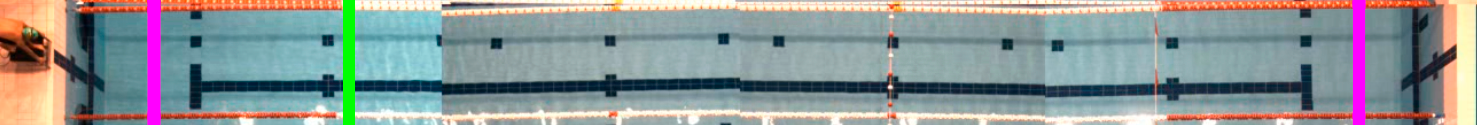
\includegraphics[width=\textwidth,height=\textheight,keepaspectratio]{imagenes/parte_graficas/limites_ROI.png}
    \caption{Límites de la región de interés. En verde se marca el inicio de la primera ROI, en morado se marcan los límites habituales para las ROI.}
    \label{fig:limitesroi}
\end{figure}

Utilizaremos la coordenada X de la esquina inferior izquierda de la bounding para distinguir el sentido de nado del nadador. Cuando el valor siga una tendencia creciente sabremos que se esta nadando de izquierda a derecha, mientras que si la tendencia es decreciente se estará nadando en el sentido contrario.

En la figura \ref{fig:diagramasecuenciacoordenadasX} se puede observar un diagrama de secuencia que resume el procedimiento que vamos a seguir. Nótese que los dos primeros pasos corresponden al preprocesamiento descrito en la sección anterior.

\begin{figure}
    \centering
    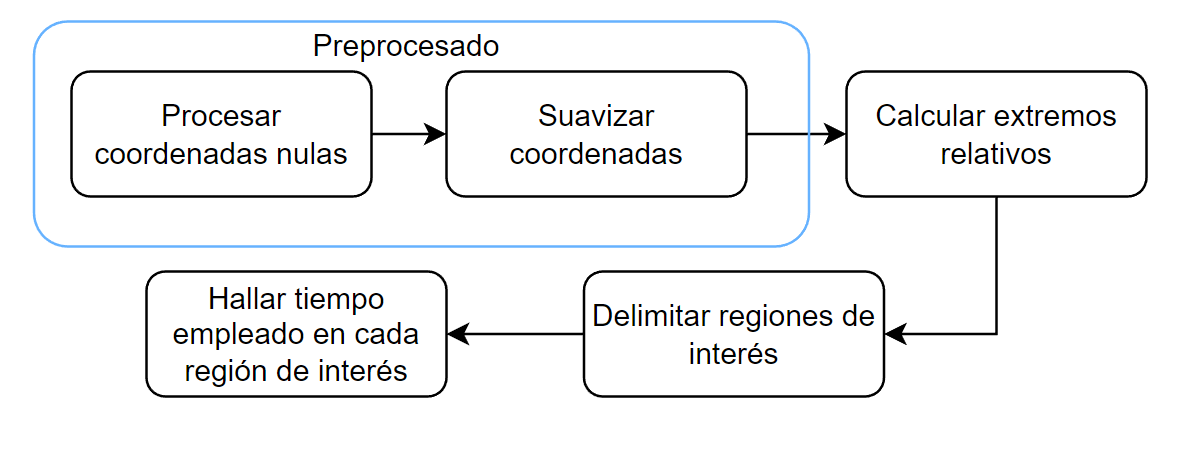
\includegraphics[width=\textwidth,height=\textheight,keepaspectratio]{imagenes/parte_graficas/Coordenada X.png}
    \caption{Secuencia de procesado de las coordenada X.}
    \label{fig:diagramasecuenciacoordenadasX}
\end{figure}

Tras haber realizado el preprocesamiento de las coordenadas X, hallaremos los extremos relativos de la función que describen. Los extremos relativos nos permiten identificar los momentos en los que el nadador cambia el sentido del nado, y por tanto se cambia de split, ya que el valor de las coordenadas X cambia de tendencia. Para ello, haremos uso de la función \textit{find\_peaks} del paquete software \textit{Scipy}. Esta función nos permite obtener los máximos relativos de una función, pero no los mínimos relativos. Para resolver este inconveniente se utiliza esta función dos veces; la primera de ellas se realiza sobre la distribución suavizada para obtener sus máximos relativos, mientras que la segunda vez se utiliza sobre la distribución suavizada multiplicada por menos uno. Los máximos relativos de la distribución cambiada de signo equivalen a los mínimos relativos de la distribución original. 

En la figura \ref{fig:ejemplocoordenadasX} se puede apreciar la evolución de la coordenada X de la esquina inferior izquierda de la bounding box. En dicha gráfica se han marcado los principales puntos de interés. Los puntos verdes indican los límites de cada split, mientras que los puntos azules indican los límites de cada región de interés. En torno al fotograma 800 se encuentra el máximo absoluto que indica el cambio de sentido de nado. 


\begin{figure}
   \centering
   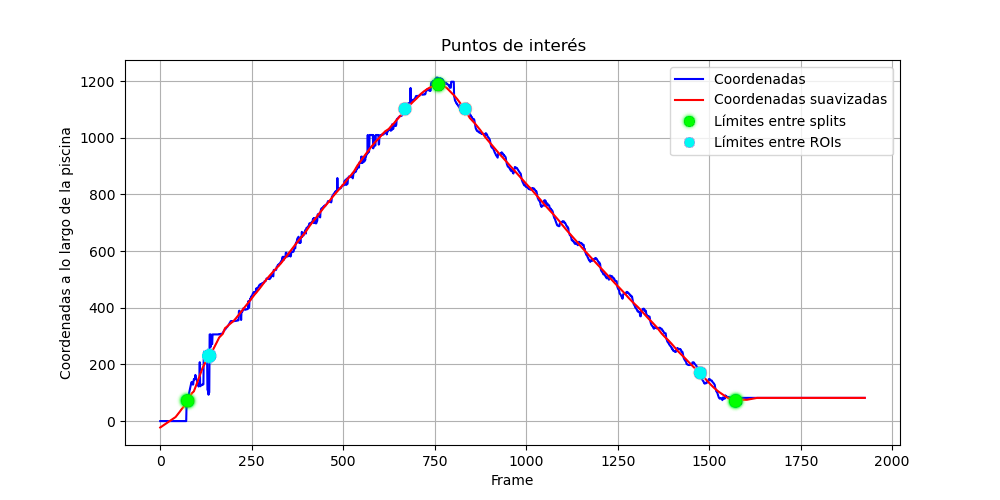
\includegraphics[width=\textwidth,height=\textheight,keepaspectratio]{imagenes/parte_graficas/SENTID.png}
   \caption{Evolución de la coordenada X y puntos de interés.}
   \label{fig:ejemplocoordenadasX}
\end{figure}

Conocidos los extremos relativos del conjunto de valores correspondientes a la coordenada X en que se encuentra el nadador, se utilizará el número de fotograma en que se producen para delimitar los splits. De esta manera, un split durará el número de fotogramas que separe un máximo y mínimo relativo consecutivos.

Esto permite delimitar los splits en los que se divide la prueba, a excepción del primero y el último. Dichos splits deben ser tratados de forma especial dado que no se pueden obtener gracias a la distancia de extremos relativos; esto es debido a que: (i) cuando se inicia el primer split los valores de la coordenada X siguen una tendencia estrictamente creciente, por lo que no existe mínimo relativo, (ii) cuando se termina el último split los valores siguen una tendencia estrictamente decreciente, por lo que no existe máximo relativo.

Para calcular el tiempo que se tarda en recorrer la región de interés en cada uno de los split delimitados, haremos uso de los números de fotograma en los que el nadador pasa por los extremos de la región de interés, cuyas posiciones son constantes y conocidas. Conocidos los fotogramas límite de las regiones de interés (ROI), hallar el tiempo empleado para recorrerlas será tan sencillo como aplicar la expresión: 

\begin{equation}
    T (s) = \frac{\text{nº fotograma final ROI} - \text{nº fotograma inicial ROI}}{ \text{tasa de fotogramas por segundo}}
\end{equation}

Tras haber delimitado las regiones de interés de cada split y haber calculado el tiempo que se tarda en recorrerlas, se debe proceder a calcular el número de brazadas que tiene lugar en cada región.

\section{Detección de brazadas y cálculo de la frecuencia media de nado} \label{sec:brazadassplit}

Como se introdujo en el capítulo \ref{cap:capitulo2}, el movimiento realizado por los brazos del nadador sigue una cierta periodicidad. Por tanto, podemos estimar el número de brazadas a partir de la variación en la anchura en el eje Y de la caja que proporcionan los métodos de detección utilizados en los capítulos anteriores. Las brazadas corresponderán a fotogramas en los que la anchura de la caja en el eje Y sea máxima, dado que el nadador debe extender los brazos hacia los lados para bracear. Este comportamiento se puede apreciar  en la figura \ref{fig:vervariacionanchura}. En dicha figura se puede apreciar claramente cómo la anchura de la caja en el eje Y aumenta conforme se extienden los brazos para realizar la brazada, y disminuye tras realizarla para volver a la posición inicial, por lo que podemos usar el momento de máxima anchura para reconocer la realización de la brazada. Este comportamiento se repite de forma periódica. Nótese que la variación de anchura concreta dependerá del estilo de nado, pero todos ellos comparten la tendencia mencionada.

\begin{figure}
    \centering
    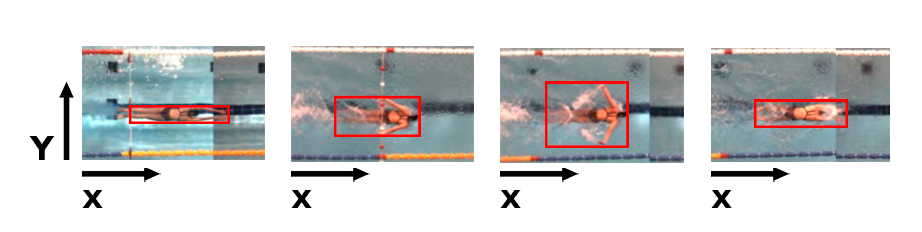
\includegraphics[width=\textwidth,height=\textheight,keepaspectratio]{imagenes/parte_graficas/variacion_anchura_nadador.png}
    \caption{Variación de anchura de la caja del nadador en el eje Y conforme se realiza una brazada.}
    \label{fig:vervariacionanchura}
\end{figure}

En la figura \ref{fig:diagramasecuenciaanchura} se muestra un diagrama de secuencia del procesado que se va a realizar sobre las anchuras del nadador en cada fotograma del vídeo, obtenidas con los métodos de detección de los capítulos \ref{cap:capitulo3} y \ref{cap:capitulo4}.

\begin{figure}
    \centering
    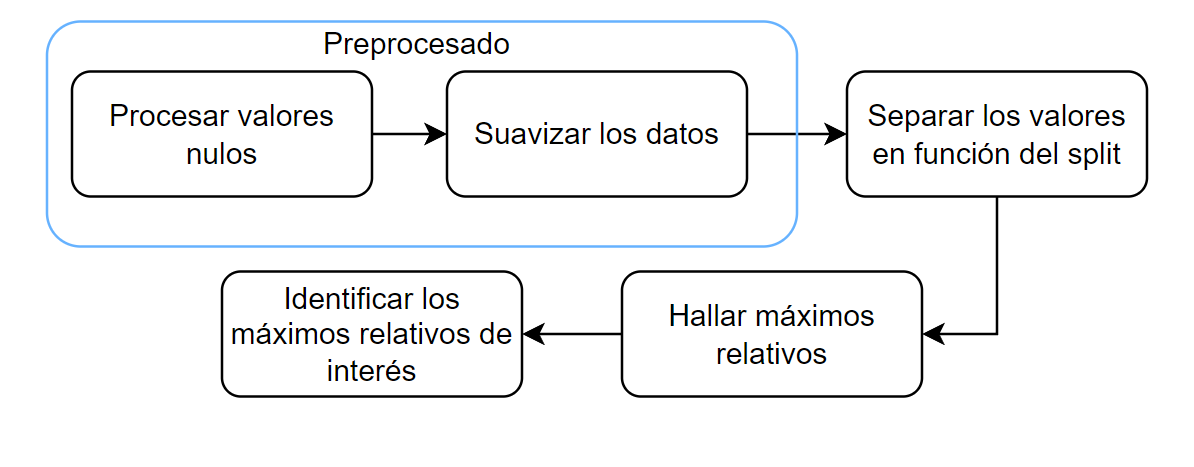
\includegraphics[width=\textwidth,height=\textheight,keepaspectratio]{imagenes/parte_graficas/Anchura.png}
    \caption{Secuencia de procesado de las anchuras de los nadadores.}
    \label{fig:diagramasecuenciaanchura}
\end{figure}

Tras haber preprocesado las anchura de las cajas, hallaremos los máximos relativos utilizando la función \textit{find\_peaks}. Sin embargo, no todos los máximos relativos nos serán de interés, pues no todos ellos corresponderán a brazadas del nadador. 

Los máximos relativos que permitirán distinguir las brazadas son aquellos de mayor valor. La función \textit{find\_peaks} permite discriminar aquellos menos relevantes e ignorarlos. Adicionalmente, impondremos la condición de que un máximo relativo pueda ser candidato a brazada sí tiene un valor mayor a la media del conjunto de valores. Este criterio se basa en el hecho de que en la mayoría de técnicas de nado los momentos de braceo son menores y de menor duración que aquellos en los que el brazo se encuentra estirado horizontalmente, con una menor anchura.

Por último, se considerarán como brazadas aquellos máximos relativos que se distancian entre sí en un determinado número mínimo de fotogramas. Esta distancia entre fotogramas es un parámetro clave, dado que permitirá obviar situaciones imposibles de realizar por un nadador, como bracear dos veces en menos de 0.2 segundos. La distancia mínima entre fotogramas utilizada para realizar esta selección es igual a la mitad de la tasa de fotogramas por segundo. Este valor fue proporcionado por los investigadores de la Facultad de Ciencias del Deporte, basándose en que ninguno de sus nadadores es capaz de realizar dos brazadas consecutivas en menos de medio segundo. 

Como se puede observar en las figuras \ref{fig:anchurasmariposa} y \ref{fig:anchurascrol}, correspondientes a nado en estilo mariposa y crol, el método propuesto permite distinguir las brazadas de una forma adecuada. También se puede apreciar cómo existen diferencias en las anchuras determinadas por los distintos detectores de objetos, existiendo un mayor nivel de ruido en las medidas obtenidas haciendo uso de GSoC. El análisis de la bondad de las predicciones realizadas con cada técnica de detección de objetos se pospone a la sección \ref{sec:resultadoscalculos}.

\begin{figure}
    \centering
    \begin{tabular}{c}
        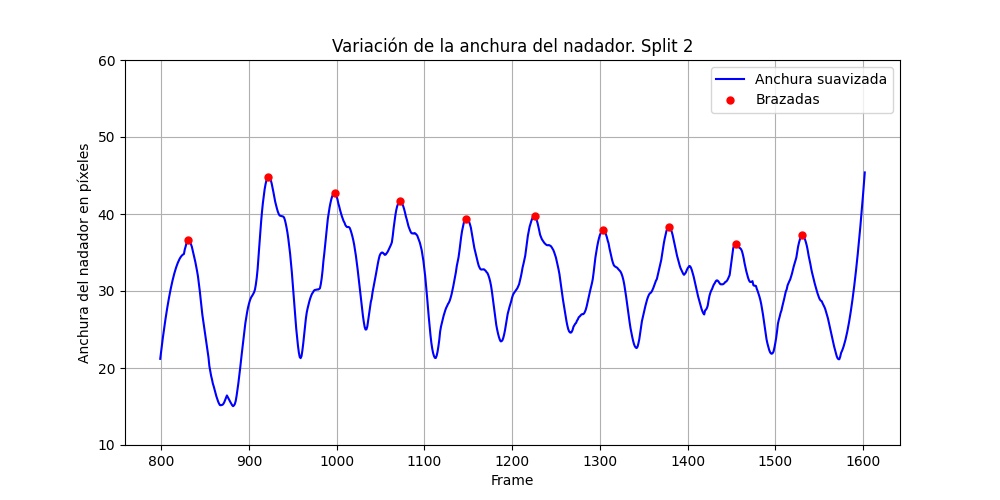
\includegraphics[width=0.6\textwidth,height=\textheight,keepaspectratio]{imagenes/parte_graficas/anchuras_calle_3_mariposa_GSoC.png}  \\
        a) Detección con GSoC. \\
         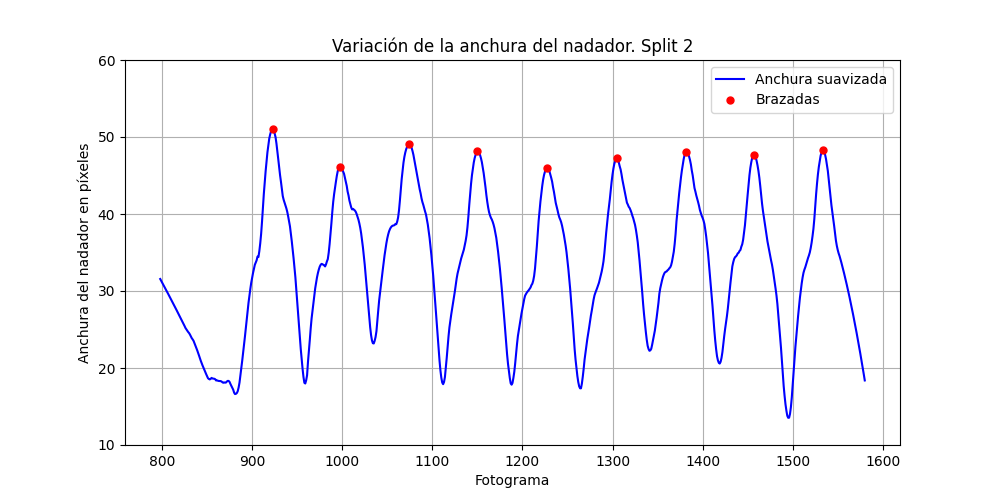
\includegraphics[width=0.6\textwidth,height=\textheight,keepaspectratio]{imagenes/parte_graficas/anchuras_calle_3_mariposa_YOLO.png} \\
        b) Detección con YOLO.
    \end{tabular}
    \caption{Anchuras para nado en mariposa.} % Split 2 calle 3.
    \label{fig:anchurasmariposa}
\end{figure}

    \begin{figure}
        \centering
        \begin{tabular}{c}
            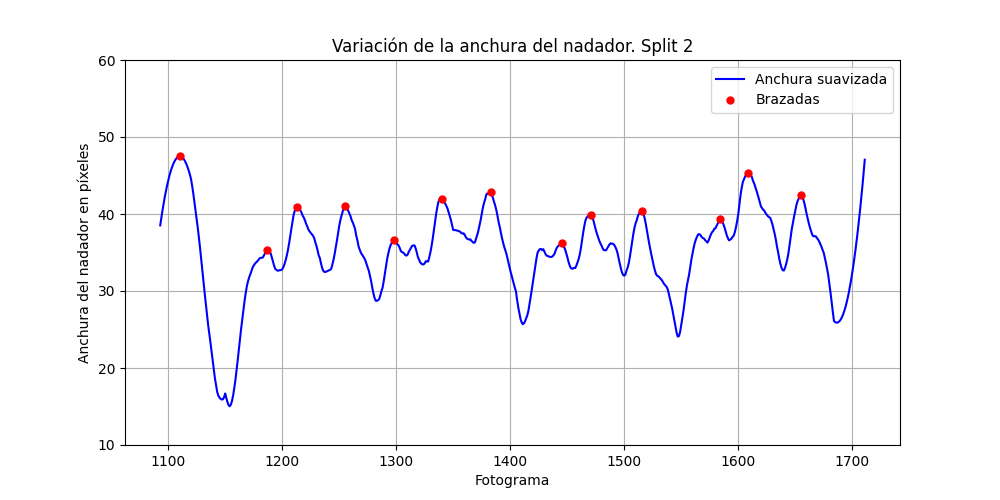
\includegraphics[width=0.6\textwidth,height=\textheight,keepaspectratio]{imagenes/parte_graficas/anchuras_calle_5_freestyle_GSoC.png}  \\
            a) Detección con GSoC. \\
             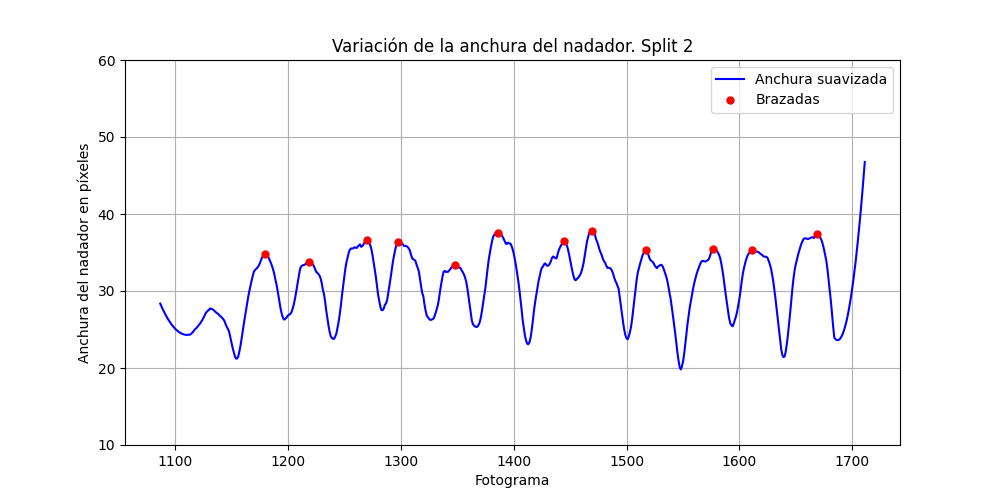
\includegraphics[width=0.6\textwidth,height=\textheight,keepaspectratio]{imagenes/parte_graficas/anchuras_calle_5_freestyle_YOLO.png} \\
            b) Detección con YOLO.
        \end{tabular}
        \caption{Anchuras para nado en crol.} % Split 2 calle 5.
        \label{fig:anchurascrol}
    \end{figure}


Una vez se conoce el tiempo que se tarda en recorrer cada región de interés, y el número de brazadas que se realiza en cada una de ellas, el cálculo de la frecuencia media de nado por split (FNMS) se reduce a:
\begin{equation}
    \text{FNMS} (brazadas/min) = \frac{ \text{número de brazadas} * \frac{\text{60 segundos}}{minuto} }{ \text{segundos en recorrer la región de interés}}
\end{equation}

Para calcular la frecuencia media de nado a lo largo de toda la prueba, bastará con calcular la media aritmética de los valores obtenidos anteriormente.

Tras haber descrito cómo calcular la frecuencia media de nado, tanto por split como para el total de la secuencia de vídeo. En la siguiente sección se mostrarán los resultados experimentales obtenidos.

\section{Evaluación experimental} \label{sec:resultadoscalculos}

Una vez que hemos presentado el modelo para el cálculo de la frecuencia media de nado analizaremos los resultados experimentales obtenidos. Para ello, vamos a comparar los datos obtenidos con cada aproximación (tiempo empleado en recorrer la región y número de brazadas) y el resultado final obtenido (FNMS).

Dado que los vídeos proporcionados por los investigadores de la Facultad de Ciencias del Deporte carecen de etiquetas, ha sido necesario etiquetarlos para realizar esta evaluación experimental. Se ha medido manualmente el tiempo que se tarda en recorrer las regiones de interés y el número de brazadas en 7 pruebas de 50 metros, de manera que tenemos 14 splits. Dado que existen diferentes estilos de nado, se han considerado dos pruebas de nado en estilo mariposa, dos en crol, dos en braza y una en espalda. Nótese que pese a que no se trata de un problema difícil, las etiquetas no provienen de un experto. 

\subsection{Estimación del tiempo empleado en recorrer una región de interés}
En primer lugar, se analizará la influencia del método de detección de objetos utilizado a la hora de realizar la estimación del tiempo que se tarda en recorrer cada región de interés.

Los tiempos estimados por cada una de las aproximaciones de los capítulos \ref{cap:capitulo3} y \ref{cap:capitulo4}, así como los tiempos reales para cada una de las pruebas se muestran en la tabla \ref{tab:tablatiemposcap5}. Todos ellos se encuentran expresados en segundos.

\begin{table}[]
    \centering
    \small
    \begin{tabular}{|c|c|c|c|} \hline
         Estilo & T. est. GSoC & T. est. YOLO & T. real  \\ \hline  
         Mariposa & 14.50 & 14.98 & 13.91  \\   
         Mariposa & 18.05 & 18.38 & 18.31 \\    
         Mariposa & 16.86 & 16.52 & 16.68 \\    
         Mariposa & 19.79 & 20.76 & 20.44 \\    
         Crol & 12.57 & 11.29 & 11.94  \\      
         Crol & 14.60 & 13.29 & 13.54 \\        
         Crol & 12.98 & 12.21 & 12.01 \\       
         Crol & 14.38 & 14.86 & 14.78 \\        
         Braza & 13.50 & 12.83 & 12.58 \\       
         Braza & 14.60 & 14.71 & 15.30 \\      
         Braza & 11.98 & 12.48 & 12.21  \\      
         Braza & 14.19 & 14.19 & 14.72  \\      
         Espalda & 15.81 & 15.31 & 15.55 \\    
         Espalda & 17.48 & 17.50 & 17.82 \\ \hline 
    \end{tabular}
    \caption{Tiempo estimado (en segundos) en recorrer cada ROI según los distintos métodos.}
    \label{tab:tablatiemposcap5}
\end{table} 

En la tabla \ref{tab:tablatiemposcap5} se puede observar cómo en ningún caso se predice correctamente el tiempo necesario para recorrer cada una de la regiones de interés. Ambos métodos discrepan en el tiempo predicho salvo en una ocasión, y no existe un patrón claro que indique que un método u otro tiende a estimar más o menos tiempo en función del estilo de nado. 

Para poder determinar que método ofrece predicciones más fiables se ha calculado el error absoluto relativo para cada caso. El error absoluto relativo es una métrica que indica la calidad de una predicción \cite{estadistica}. Este se define cómo:

\begin{equation}
    Error_{\text{absoluto relativo}} = \frac{|Valor_{real} - Valor_{predicho}|}{Valor_{real}}
\end{equation}

Utilizaremos esta métrica ya que nos indica la proporción del error con respecto al valor exacto de la medición, permitiéndonos comparar los errores que se producen en distintas pruebas. Nótese que no sería igual cometer un error de predicción de 2 segundos en una prueba de nado de 10 segundos, que en una prueba que durase una hora.

Esta información se puede consultar en la tabla \ref{tab:tablaerrorestiemposcap5}. Para obtener una visión más general en función del estilo de nado, se han calculado los errores relativos medios para cada uno de ellos, así como el error absoluto relativo medio total. Estos valores se pueden consultar en la tabla \ref{tab:tablatiemposmedioscap5}. Nótese que el error absoluto relativo es muy pequeño en todos los casos, por lo que ambas técnicas realizan una predicción del tiempo empleado en recorrer la ROI bastante precisa. Sin embargo, YOLO ofrece menor error absoluto relativo para todos los estilos de nado a excepción de mariposa, así como un menor error absoluto relativo  medio total. Por tanto, se puede concluir que YOLO ofrece mejores predicciones del tiempo que se tarda en recorrer cada región de interés.

\begin{table}[]
    \centering
    \small
    \begin{tabular}{|c|c|c|} \hline
         Estilo & Err. relatv. GSoC & Err. relatv. YOLO  \\ \hline 
         Mariposa & \textbf{0.04241} & 0.07692 \\
         Mariposa & 0.01420 & \textbf{0.00382} \\
         Mariposa & 0.01080 & \textbf{0.00959} \\
         Mariposa & 0.03180 & \textbf{0.01565} \\
         Crol & \textbf{0.05276} & 0.05444 \\
         Crol & 0.07829 & \textbf{0.01846} \\
         Crol & 0.08076 & \textbf{0.01665} \\
         Crol & 0.02706 & \textbf{0.00541} \\
         Braza & 0.07313 & \textbf{0.01987} \\
         Braza & 0.04575 & \textbf{0.03856} \\
         Braza & \textbf{0.01884} & 0.02211 \\
         Braza & 0.03600 & 0.03600 \\
         Espalda & 0.01672 & \textbf{0.01543} \\
         Espalda & 0.01908 & \textbf{0.01796} \\ \hline
    \end{tabular}
    \caption{Error absoluto relativo en las predicciones del tiempo empleado para recorrer cada ROI según los distintos métodos. }
    \label{tab:tablaerrorestiemposcap5}
\end{table}

\begin{table}[]
    \centering
    \small
    \begin{tabular}{|c|c|c|} \hline
         Estilo & Err. relatv. medio GSoC & Err. relatv. medio YOLO  \\ \hline
         Mariposa & \textbf{0.024803} & 0.026495 \\
         Crol & 0.061423 & \textbf{0.02374}  \\   
         Braza & 0.043430 & \textbf{0.029135} \\
         Espalda & 0.017900 & \textbf{0.016695} \\
         Media & 0.039603 & \textbf{0.025062} \\ \hline
    \end{tabular}
    \caption{Comparativa entre los errores relativos medios de los tiempos estimados.}
    \label{tab:tablatiemposmedioscap5}
\end{table} 

\subsection{Estimación del número de brazadas }
El número de brazadas estimado por cada una de las aproximaciones de los capítulos \ref{cap:capitulo3} y \ref{cap:capitulo4} se muestra en \ref{tab:tablabrazadascap5}.

\begin{table}[]
    \centering
    \small
    \begin{tabular}{|c|c|c|c|} \hline
         Estilo & Br. est. GSoC & Br. est. YOLO & Br. reales  \\ \hline
         Mariposa & 9 & 9 & 9  \\   
         Mariposa & 10 & 9 & 9 \\
         Mariposa & 11 & 11 & 11 \\
         Mariposa & 12 & 12 & 13 \\
         Crol & 8 & 8 & 8  \\
         Crol & 10 & 9 & 9 \\
         Crol & 9 & 11 & 11 \\  
         Crol & 13 & 12 & 12 \\
         Braza & 14 & 9 & 9 \\  
         Braza & 9 & 9 & 9 \\
         Braza & 9 & 10 & 10  \\
         Braza & 11 & 13 & 12  \\
         Espalda & 10 & 11 & 12 \\
         Espalda & 8 & 13 & 13 \\ \hline
    \end{tabular}
    \caption{Comparativa entre brazadas estimadas y reales.}
    \label{tab:tablabrazadascap5}
\end{table}


Analicemos los resultados presentados para cada estilo de nado. 
\begin{itemize}
    \item Para el nado en estilo crol, GSoC solamente es capaz de estimar el número de brazadas correcto en una ocasión. Para el segundo y cuarto caso estima una brazada de más, mientras que para el tercer caso estima dos brazadas menos. Sin embargo, se puede observar que YOLO es capaz de predecir correctamente el número de brazadas en todas las ocasiones.
    
    \item Para el nado en estilo mariposa, GSoC es capaz de estimar correctamente el número de brazadas realizadas en el primer y tercer caso, mientras que para el segundo caso estima una brazada de más y para el cuarto caso una brazada de menos. YOLO es capaz de predecir correctamente en tres de los cuatro casos analizados, estimando una brazada menos en el cuarto. Ambos métodos tienen dificultades para reconocer brazadas cuando estás se realizan muy cerca del final de la región de interés.
    
    \item Para el nado en braza, GSoC solamente es capaz de estimar correctamente en el segundo caso. Resulta especialmente notable el error cometido en el primer caso, donde se estiman 5 brazadas más de las realmente realizadas. Por otra parte, YOLO es capaz de acertar la predicción en los tres primeros casos, mientras que en el cuarto estima una brazada de más.
    
    \item Para el nado en espalda, GSoC no es capaz de acertar ninguna de las dos predicciones. Para el segundo caso, el error cometido es bastante notable, al estimar 5 brazadas menos de las realmente realizadas. YOLO es capaz de acertar la segunda predicción, mientras que en la primera estima una brazada de menos.
\end{itemize}

En la tabla \ref{tab:tablaerroresbrazadascap5} se muestra el error absoluto relativo cometido por cada aproximación a la hora de estimar el número de brazadas que tienen lugar en cada región de interés. Como se puede observar rápidamente, la aproximación propuesta en el capítulo \ref{cap:capitulo3} presenta un mayor error absoluto relativo que la aproximación propuesta en el capítulo \ref{cap:capitulo4} en la mayoría de casos donde no es capaz de acertar el número de brazadas realizadas. En la tabla \ref{tab:tablaerroresmediosbrazadas} se presentan los errores relativos medios en función del estilo de nado y el error absoluto relativo medio total. El detector YOLO ofrece un error absoluto relativo medio menor en todos los estilos de nado, siendo este capaz de no cometer ningún error a la hora de predecir brazadas en estilo crol. Nótese que el detector GSoC sufre especialmente a la hora de detectar brazadas del nadador en estilo braza y de espalda. 

\begin{table}[]
    \centering
    \small
    \begin{tabular}{|c|c|c|} \hline
         Estilo & Err. relatv. GSoC & Err. relatv. YOLO  \\ \hline 
         Mariposa & 0 & 0 \\
         Mariposa & 0.1111 & \textbf{0} \\
         Mariposa & 0 & 0 \\
         Mariposa & 0.0833 & 0.0833 \\
         Crol & 0 & 0 \\
         Crol & 0.1111 & \textbf{0} \\
         Crol & 0.1818 & \textbf{0} \\
         Crol & 0.0833 & \textbf{0} \\
         Braza & 0.5555 & \textbf{0} \\
         Braza & 0 & 0 \\
         Braza & 0.1000 & \textbf{0} \\
         Braza & 0.0833 & 0.0833 \\
         Espalda & 0.1666 & \textbf{0.0833} \\
         Espalda & 0.3846 & \textbf{0} \\ \hline
    \end{tabular}
    \caption{Error absoluto relativo en las predicciones del número de brazadas realizadas.} 
    \label{tab:tablaerroresbrazadascap5}
\end{table}

\begin{table}[]
    \centering
    \small
    \begin{tabular}{|c|c|c|} \hline
         Estilo & Err. relatv. medio GSoC & Err. relatv. medio YOLO  \\ \hline
         Mariposa & 0.0486 & \textbf{0.0208} \\
         Crol & 0.0941 & \textbf{0}  \\   
         Braza & 0.1847 & \textbf{0.0208} \\
         Espalda & 0.2765 & \textbf{0.0417} \\
         Media & 0.1330 & \textbf{0.0178} \\ \hline
    \end{tabular}
    \caption{Comparativa entre los errores relativos medios del número de brazadas estimadas.}
    \label{tab:tablaerroresmediosbrazadas}
\end{table} 

\subsection{Estimación de la frecuencia de nado media}

Una vez hemos comprobado la bondad en las estimaciones del tiempo que se emplea en recorrer un split y el número de brazadas realizadas, comprobamos que efecto tienen dichas estimaciones en el cálculo de la FNMS. A partir de los valores anteriores, en la tabla \ref{tab:frecuenciasmedianadoest} se muestran las frecuencias medias de nado estimadas y reales medidas en brazadas por minuto. Nótese que las frecuencias medias de nado reales han sido calculadas a partir de mediciones realizadas manualmente para cada vídeo, ya que los investigadores de la Facultad de Ciencias del Deporte no indicaron valores de referencia.

\begin{table}[]
    \centering
    \small
    \begin{tabular}{|c|c|c|c|} \hline
         Estilo & Est. GSoC & Est. YOLO & Valores reales  \\ \hline
         Mariposa & 37.24 & 36.06 & 38.82  \\   
         Mariposa & 33.25 & 29.38 & 29.49 \\
         Mariposa & 39.15 & 39.94 & 39.10 \\
         Mariposa & 36.39 & 34.68 & 38.16 \\
         Crol & 38.18 & 42.53 & 40.20  \\   
         Crol & 41.11 & 40.65 & 39.88 \\    
         Crol & 41.61 & 54.04 & 54.95 \\    
         Crol & 54.24 & 48.46 & 48.71 \\    
         Braza & 62.22 & 42.08 & 42.93 \\   
         Braza & 37.00 & 36.70 & 35.29 \\   
         Braza & 45.09 & 48.09 & 49.14  \\  
         Braza & 46.51 & 54.97 & 48.91  \\  
         Espalda & 37.95 & 43.11 & 46.30 \\ 
         Espalda & 27.47 & 44.57 & 43.77 \\ \hline 
    \end{tabular}
    \caption{Comparativa entre frecuencias medias de nado estimadas y reales.}
    \label{tab:frecuenciasmedianadoest}
\end{table}

En la tabla \ref{tab:tablaerroresprediccionesfrecuencia} se muestran los errores relativos para cada una de las pruebas evaluadas, remarcando en negrita el menor error absoluto relativo en cada caso. Por otra parte, en la tabla \ref{tab:tablaerroresmediosprediccionesfrecuencia} se muestran los errores relativos medios para cada uno de los estilos de nado, así como el error absoluto relativo medio total.

\begin{table}[]
    \centering
    \small
    \begin{tabular}{|c|c|c|} \hline
         Estilo & Err. relatv. GSoC & Err. relatv. YOLO  \\ \hline 
         Mariposa & \textbf{0.0407} & 0.0711 \\
         Mariposa & 0.1275 & \textbf{0.0031} \\
         Mariposa & \textbf{0.0013} & 0.0215 \\
         Mariposa & \textbf{0.0464} & 0.0912 \\
         Crol & \textbf{0.05024} & 0.05796 \\
         Crol & 0.03084 & \textbf{0.01931} \\
         Crol & 0.24277 & \textbf{0.01656} \\
         Crol & 0.11353 & \textbf{0.00513} \\
         Braza & 0.44933 & \textbf{0.01980} \\
         Braza & 0.04845 & \textbf{0.03995} \\
         Braza & 0.08302 & \textbf{0.02136} \\
         Braza & \textbf{0.04907} & 0.12390 \\
         Espalda & 0.18034 & \textbf{0.06889} \\
         Espalda & 0.37240 & \textbf{0.01827} \\ \hline
    \end{tabular}
    \caption{Error absoluto relativo en las predicciones de la frecuencia media de nado.}
    \label{tab:tablaerroresprediccionesfrecuencia}
\end{table}

\begin{table}[]
    \centering
    \small
    \begin{tabular}{|c|c|c|} \hline
         Estilo & Err. relatv. medio GSoC & Err. relatv. medio YOLO  \\ \hline
         Mariposa & 0.0540 & \textbf{0.0467} \\
         Crol & 0.1093 & \textbf{0.0247}  \\   
         Braza & 0.1574 & \textbf{0.0417} \\
         Espalda & 0.2764 & \textbf{0.0436} \\
         Media & 0.1311 & \textbf{0.0385} \\ \hline
    \end{tabular}
    \caption{Comparativa entre los errores relativos medios de las frecuencias medias de nado estimadas.}
    \label{tab:tablaerroresmediosprediccionesfrecuencia}
\end{table} 

Como se puede observar en la tabla \ref{tab:tablaerroresmediosprediccionesfrecuencia}, YOLO ofrece un menor error absoluto relativo medio en todas los estilos de nado. A excepción del estilo mariposa, YOLO ofrece una reducción bastante considerable de los errores relativos con respecto de GSoC. Se puede observar que el error absoluto relativo medio total de YOLO es unas 3.4 veces menor, aproximadamente. Esto es un indicativo de que las predicciones realizadas por YOLO se acercan más a la realidad que las realizadas por GSoC.

En virtud de los experimentos realizados, se puede concluir que el método propuesto es capaz de predecir con un buen nivel de acierto tanto el tiempo que se tarda en recorrer una región de interés como el número de brazadas que hicieron falta para ello, y por tanto, la frecuencia media de nado. En concreto, los experimentos indican que YOLO ofrece un rendimiento superior frente a GSoC al realizar la estimación de la frecuencia media de nado con nivel de error considerablemente menor.
